% !TeX program = xelatex
\documentclass[12pt,a4paper,oneside]{report}

% ======================== FIELDS TO UPDATE ========================
\newcommand{\University}{HANOI UNIVERSITY OF SCIENCE AND TECHNOLOGY}
\newcommand{\School}{SCHOOL OF INFORMATION AND COMMUNICATION TECHNOLOGY}
\newcommand{\CourseName}{PROJECT 1}
\newcommand{\ReportTitle}{A RAG-ENHANCED SYSTEM FOR JOB DESCRIPTION AUTHORING AND INTERVIEW QUESTION GENERATION}
\newcommand{\ProjectName}{SmartHire Composer}
\newcommand{\StudentName}{NGUYEN QUAN}
\newcommand{\StudentID}{STUDENT ID}
\newcommand{\ClassName}{CLASS / TRAINING PROGRAM}
\newcommand{\Supervisor}{SUPERVISOR NAME}
\newcommand{\Semester}{Semester 2025.2}
\newcommand{\PlaceAndDate}{Hanoi, June 2026}
% ==================================================================

\usepackage{fontspec}
\IfFontExistsTF{Times New Roman}{\setmainfont{Times New Roman}}{\setmainfont{Tinos}}
\IfFontExistsTF{Arial}{\setsansfont{Arial}}{\setsansfont{Arimo}}
\IfFontExistsTF{Consolas}{\setmonofont{Consolas}}{\setmonofont{DejaVu Sans Mono}}
\usepackage[english]{babel}
\usepackage{geometry}
\geometry{top=2.5cm,bottom=2.5cm,left=3.2cm,right=2.2cm}
\usepackage{setspace}
\onehalfspacing
\usepackage{indentfirst}
\setlength{\parindent}{1.27cm}
\setlength{\parskip}{3pt}
\usepackage{graphicx}
\usepackage{booktabs,longtable,array,multirow,tabularx}
\usepackage{amsmath,amssymb}
\usepackage{enumitem}
\usepackage{caption,subcaption}
\usepackage{float}
\usepackage{xcolor}
\usepackage{listings}
\usepackage{tikz}
\usetikzlibrary{arrows.meta,positioning,shapes.geometric,fit,calc}
\usepackage{fancyhdr}
\usepackage{titlesec}
\usepackage{hyperref}
\usepackage{bookmark}
\usepackage{url}

\definecolor{HustRed}{RGB}{180,30,45}
\definecolor{CodeBg}{RGB}{247,248,250}
\definecolor{CodeBlue}{RGB}{29,78,216}
\hypersetup{colorlinks=true,linkcolor=black,citecolor=CodeBlue,urlcolor=CodeBlue,pdfauthor={\StudentName},pdftitle={\ReportTitle}}
\captionsetup{font=small,labelfont=bf,labelsep=period}

\renewcommand{\contentsname}{TABLE OF CONTENTS}
\renewcommand{\listfigurename}{LIST OF FIGURES}
\renewcommand{\listtablename}{LIST OF TABLES}
\renewcommand{\bibname}{REFERENCES}

\titleformat{\chapter}[hang]{\bfseries\large}{CHAPTER \thechapter.}{0.6em}{\MakeUppercase}
\titlespacing*{\chapter}{0pt}{-20pt}{20pt}
\titleformat{\section}{\bfseries\large}{\thesection}{0.6em}{}
\titleformat{\subsection}{\bfseries\normalsize}{\thesubsection}{0.6em}{}

\pagestyle{fancy}
\setlength{\headheight}{14pt}
\fancyhf{}
\fancyhead[L]{\small \CourseName}
\fancyhead[R]{\small \ProjectName}
\fancyfoot[C]{\thepage}
\renewcommand{\headrulewidth}{0.4pt}

\lstset{
  basicstyle=\ttfamily\small,
  backgroundcolor=\color{CodeBg},
  frame=single,
  rulecolor=\color{gray!35},
  breaklines=true,
  columns=fullflexible,
  keywordstyle=\color{CodeBlue}\bfseries,
  commentstyle=\color{green!45!black},
  stringstyle=\color{orange!60!black},
  showstringspaces=false,
  numbers=left,
  numberstyle=\tiny\color{gray},
  xleftmargin=1.4em,
  framexleftmargin=1em
}

\newcommand{\keyword}[1]{\textbf{Keywords:} #1}
\newcommand{\code}[1]{\texttt{#1}}
\newcommand{\todoField}[1]{\textcolor{HustRed}{\textbf{[#1]}}}

\begin{document}

% ============================== COVER ==============================
\begin{titlepage}
\begin{center}
{\bfseries\large \University\\[0.25cm] \School}\par
\vspace{1.1cm}

\begin{tikzpicture}
\draw[HustRed, line width=1.5pt] (0,0) circle (1.1cm);
\node[align=center,text=HustRed,font=\bfseries] at (0,0) {SOICT\\HUST};
\end{tikzpicture}
\vspace{0.8cm}

{\bfseries\LARGE \CourseName{} REPORT}\par
\vspace{1.0cm}
{\bfseries\large TOPIC:}\par
\vspace{0.35cm}
\begin{minipage}{0.92\textwidth}
\centering
{\bfseries\Large\color{HustRed} \ReportTitle}
\end{minipage}
\vfill

\begin{tabular}{>{\bfseries}p{4.8cm}p{9.2cm}}
Student: & \StudentName\\[0.25cm]
Student ID: & \StudentID\\[0.25cm]
Class / program: & \ClassName\\[0.25cm]
Supervisor: & \Supervisor\\[0.25cm]
Semester: & \Semester
\end{tabular}
\vfill
{\bfseries \PlaceAndDate}
\end{center}
\end{titlepage}

\pagenumbering{roman}

\chapter*{DECLARATION}
\addcontentsline{toc}{chapter}{Declaration}
I, \StudentName, student ID \StudentID, hereby declare that this \CourseName{} report entitled ``\ReportTitle'' is the result of my own study, system design, implementation, and evaluation under the supervision of \Supervisor. The system metrics, test results, and implementation descriptions reported in this document were collected from the developed prototype at the time of writing. External algorithms, technical documents, libraries, and official specifications used in the project are cited in the References section. I do not submit copied work as my own result, and I take full responsibility for the integrity of this report.

\vspace{1cm}
\begin{flushright}
Hanoi, day \ldots{} month \ldots{} year 2026\\[1.8cm]
\textbf{Student}\\[1.5cm]
\StudentName
\end{flushright}

\chapter*{ACKNOWLEDGEMENTS}
\addcontentsline{toc}{chapter}{Acknowledgements}
I would like to express my sincere gratitude to \Supervisor{} for providing guidance, technical feedback, and methodological direction throughout this Project 1. I also thank the lecturers of the \School{} for the foundational knowledge in software engineering, databases, machine learning, and information systems that made this project possible. Finally, I am grateful to my family and friends for their support and encouragement during the design, implementation, testing, and documentation of this system. Any remaining shortcomings in this report are my responsibility and will serve as the basis for future improvement.

\chapter*{ABSTRACT}
\addcontentsline{toc}{chapter}{Abstract}
Recruitment teams need consistent job descriptions, explicit evaluation criteria, and role-specific interview questions. In practice, job description authoring is often fragmented across old templates, manual notes, and inconsistent role taxonomies. This makes the process time-consuming, difficult to standardize, and hard to trace. Large language models can accelerate drafting, but using them without enterprise context may produce generic or unsupported content. This report presents \ProjectName, a web-based system for creating, editing, versioning, exporting, and improving job descriptions, as well as generating interview questions. The system applies Retrieval-Augmented Generation (RAG) to ground AI-assisted writing in a curated corpus of public job postings.

The proposed solution consists of a React/Vite frontend, a FastAPI backend, PostgreSQL for transactional data and full-text retrieval, Milvus for vector search, and Gemini models for text generation and embeddings. Public ATS postings are normalized with provenance metadata, segmented into overlapping chunks, and embedded into 768-dimensional vectors. At query time, dense cosine retrieval and PostgreSQL lexical retrieval are fused using Reciprocal Rank Fusion, followed by diversity-aware selection to reduce repeated chunks from the same job description. The system also includes JWT authentication, role-based access control, version history, PDF/DOCX export, and graceful fallback when the LLM service is unavailable.

The experimental corpus contains 75 public job descriptions from three companies and 589 indexed chunks. On a 15-query self-retrieval benchmark, the hybrid retrieval pipeline achieved Recall@5 of 1.000, Mean Reciprocal Rank of 0.9556, and a unique-document ratio of 1.000. Five automated backend tests passed, the frontend production build completed successfully, and npm audit reported no known vulnerabilities. These results demonstrate that the proposed architecture is feasible for Project 1, while also identifying the need for expert-labeled relevance evaluation, larger-scale testing, production monitoring, and deeper integration with recruitment workflows in future work.

\keyword{RAG, job description, recruitment, semantic search, hybrid retrieval, Gemini, Milvus, FastAPI.}

\tableofcontents
\listoffigures
\listoftables

\chapter*{LIST OF EQUATIONS}
\addcontentsline{toc}{chapter}{List of Equations}
\begin{longtable}{p{3cm}p{11cm}}
\toprule
\textbf{Equation} & \textbf{Description}\\
\midrule
\ref{eq:cosine} & Cosine similarity between a query vector and a document vector\\
\ref{eq:rrf} & Reciprocal Rank Fusion score\\
\ref{eq:diversity} & Diversity-aware selection score with Jaccard penalty\\
\ref{eq:mrr} & Mean Reciprocal Rank\\
\bottomrule
\end{longtable}

\chapter*{LIST OF ABBREVIATIONS}
\addcontentsline{toc}{chapter}{List of Abbreviations}
\begin{longtable}{p{3cm}p{11cm}}
\toprule
\textbf{Abbreviation} & \textbf{Meaning}\\
\midrule
AI & Artificial Intelligence\\
API & Application Programming Interface\\
ATS & Applicant Tracking System\\
CRUD & Create, Read, Update, Delete\\
DBMS & Database Management System\\
ECR & Elastic Container Registry\\
ECS & Elastic Container Service\\
EKS & Elastic Kubernetes Service\\
FTS & Full-Text Search\\
HNSW & Hierarchical Navigable Small World\\
JD & Job Description\\
JWT & JSON Web Token\\
LLM & Large Language Model\\
MMR & Maximal Marginal Relevance\\
MRR & Mean Reciprocal Rank\\
RAG & Retrieval-Augmented Generation\\
RBAC & Role-Based Access Control\\
REST & Representational State Transfer\\
RRF & Reciprocal Rank Fusion\\
UI & User Interface\\
UX & User Experience\\
\bottomrule
\end{longtable}

\clearpage
\pagenumbering{arabic}

% ============================== CHAPTER 1 ==============================
\chapter{INTRODUCTION}

\section{Problem Statement}
A job description is a central artifact in the recruitment process. It communicates the hiring need, defines responsibilities and requirements, guides candidate screening, and provides the basis for building interview questions. However, in many organizations, job descriptions are written from scattered templates, old postings, and the personal experience of recruiters or hiring managers. This practice causes three major issues. First, the structure and terminology of job descriptions are often inconsistent across departments. Second, recruiters may find it difficult to reuse relevant historical examples from a large internal library. Third, when a large language model is used without appropriate context, the generated content may be too generic or may contain unsupported claims.

Retrieval-Augmented Generation (RAG) addresses part of this problem by combining information retrieval with text generation. Instead of asking an LLM to generate an answer only from its model parameters, the system first retrieves relevant passages from an external knowledge base and then injects them into the prompt. In this project, the retrieved knowledge consists of real job-description chunks with source metadata. RAG does not eliminate all LLM errors, but it improves domain grounding, enables source traceability, and separates knowledge updates from model training \cite{lewis2020rag}.

\section{Objectives and Scope}
The goal of this project is to build a web-based prototype that supports the core lifecycle of a job description. The specific objectives are: (i) collecting and normalizing public job postings with provenance information; (ii) supporting both semantic and keyword search over the job-description corpus; (iii) using retrieved context to support job-description generation and improvement; (iv) generating interview questions based on position, seniority, and competency areas; (v) managing users, access control, and job-description version history; and (vi) quantitatively evaluating retrieval quality.

The scope of Project 1 focuses on a working prototype in a development environment. The experimental corpus contains 75 public job descriptions collected from Cloudflare, Datadog, and Figma. The system does not process real candidate profiles, does not make hiring decisions, and does not collect personal information from application forms. Public ATS APIs and openly accessible job-posting metadata are prioritized. Sources that require authentication, block automated access, or disallow crawling are outside the scope of data collection.

\section{Solution Direction}
The proposed solution follows a multi-layer client-server architecture. The React frontend provides the user interface for composing job descriptions, previewing Markdown content, viewing versions, retrieving similar job descriptions, and exporting documents. The FastAPI backend provides REST APIs and coordinates business logic. PostgreSQL stores transactional data and supports lexical full-text search. Milvus stores dense embedding vectors for semantic search. Gemini models are used for both text generation and embeddings.

The retrieval pipeline combines dense retrieval with lexical retrieval. Dense retrieval captures semantic similarity, while lexical retrieval preserves exact keyword matching for skills, tool names, job titles, and rare expressions. The two ranked lists are fused using Reciprocal Rank Fusion (RRF), and a diversity-aware selection step limits repeated chunks from the same job description. This design makes the system more robust than a pure vector search or pure keyword search approach.

\begin{figure}[H]
\centering
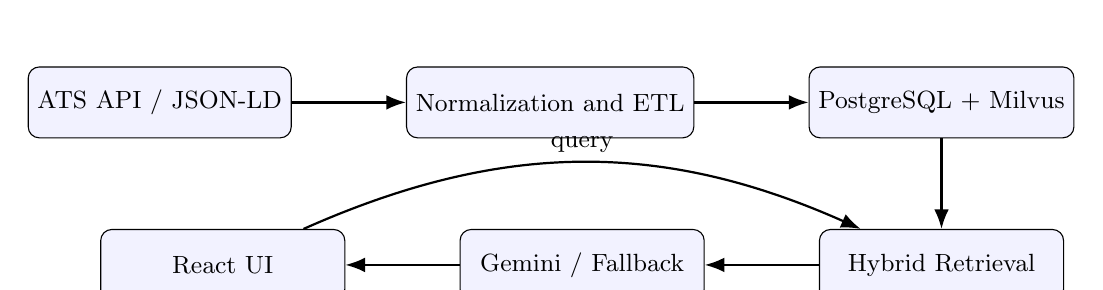
\begin{tikzpicture}[node distance=1.15cm and 1.45cm, every node/.style={font=\small}, box/.style={draw,rounded corners,minimum width=3.1cm,minimum height=0.9cm,align=center,fill=blue!5}, arr/.style={-{Latex[length=2.5mm]},thick}]
\node[box] (source) {ATS API / JSON-LD};
\node[box,right=of source] (etl) {Normalization and ETL};
\node[box,right=of etl] (store) {PostgreSQL + Milvus};
\node[box,below=of store] (retrieve) {Hybrid Retrieval};
\node[box,left=of retrieve] (llm) {Gemini / Fallback};
\node[box,left=of llm] (ui) {React UI};
\draw[arr] (source)--(etl);
\draw[arr] (etl)--(store);
\draw[arr] (store)--(retrieve);
\draw[arr] (retrieve)--(llm);
\draw[arr] (llm)--(ui);
\draw[arr,bend left=24] (ui) to node[above]{query} (retrieve);
\end{tikzpicture}
\caption{High-level processing direction of the proposed system}
\label{fig:overview-flow}
\end{figure}

\section{Main Contributions}
This project contributes a prototype that integrates several components that are often handled separately: real job-posting ingestion with provenance, versioned job-description management, hybrid RAG, AI-assisted writing, interview-question generation, role-based access control, and a usable web interface. The main technical contribution is a retrieval architecture that keeps PostgreSQL and Milvus synchronized through stable chunk identifiers, records an embedding/index manifest, combines dense and lexical ranking through RRF, and applies a per-document diversity constraint. As a result, the system is not merely an LLM wrapper; it is a traceable data-to-retrieval-to-generation pipeline that can be tested and reproduced.

\section{Report Structure}
The remainder of this report is organized as follows. Chapter 2 analyzes the current situation, user roles, functional requirements, and non-functional requirements. Chapter 3 presents the theoretical background and technologies used in the project. Chapter 4 describes system design, data modeling, the RAG pipeline, and implementation details. Chapter 5 reports the experimental setup, retrieval evaluation, software testing, and discussion of limitations. Chapter 6 concludes the report and proposes future development directions.

% ============================== CHAPTER 2 ==============================
\chapter{REQUIREMENT ANALYSIS}

\section{Current Situation}
Traditional document editors can store job-description templates, but they do not provide semantic retrieval over a growing job-description library. Standalone LLM tools can generate content quickly, but they usually lack enterprise-specific context, provenance tracking, version control, and access control. Keyword-based search systems are reliable when the query terms exactly match the stored documents, but they may fail when users describe a role in different words. These observations motivate a combined approach: a transactional database for business data, lexical retrieval for rare and exact terms, dense retrieval for semantic similarity, and LLM generation only after relevant context has been retrieved.

\section{Actors and User Roles}
The system supports four conceptual roles. The \textit{Admin} manages users, roles, and all system-level functions. The \textit{Recruiter} creates job descriptions, improves content, generates interview questions, saves versions, and exports documents. The \textit{Hiring Manager} reviews job descriptions, checks version history, and uses retrieval results to compare similar roles. The \textit{Viewer} role is intended for read-only access in future extensions.

\section{Functional Requirements}
\begin{longtable}{p{1.2cm}p{4.5cm}p{8.2cm}}
\caption{Functional requirements of the system}\label{tab:functional}\\
\toprule
\textbf{ID} & \textbf{Function} & \textbf{Description}\\
\midrule
F01 & Authentication & Users log in with username and password, receive a JWT, and retrieve the current profile.\\
F02 & JD authoring & Users enter title, department, level, job family, and language to create a draft.\\
F03 & Version management & Each saved edit is recorded with version number, author, timestamp, and change summary.\\
F04 & AI improvement and suggestions & The system improves the whole JD or suggests content for a selected section.\\
F05 & Interview-question generation & The system generates technical, behavioral, and situational questions with competency, difficulty, and rubric.\\
F06 & Retrieval & Users search in dense, lexical, or hybrid mode; filter by company or department; and receive snippet and source URL.\\
F07 & Export & The current JD can be exported to PDF or DOCX.\\
F08 & Data ingestion & The system collects job postings from Greenhouse, Lever, or JSON-LD sources and stores provenance.\\
F09 & Indexing & The system chunks documents, generates embeddings, writes vectors to Milvus, and stores a catalog in PostgreSQL.\\
F10 & Monitoring & Liveness, readiness, and request identifiers are provided for debugging and operations.\\
\bottomrule
\end{longtable}

\section{Main Business Workflow}
The main workflow begins when a recruiter logs in and enters metadata for a position. The backend builds a query from the title, level, department, and job family. The hybrid retriever returns relevant chunks with company, title, and source URL. The LLM orchestrator wraps external text inside an \code{UNTRUSTED\_SOURCE} block, instructs the model not to execute instructions from that source, and generates a grounded draft. The job description and its first version are stored. The user can then edit the Markdown content, save a new version, generate suggestions, improve the text, and export the result.

\begin{figure}[H]
\centering
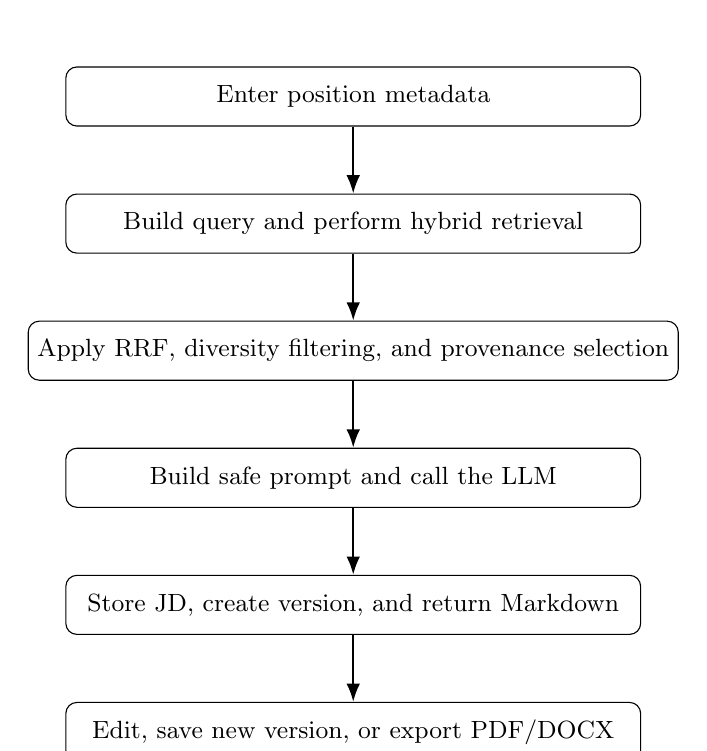
\begin{tikzpicture}[node distance=0.85cm, every node/.style={font=\small}, flowstep/.style={draw,rounded corners,minimum width=7.3cm,minimum height=0.75cm,align=center}, arr/.style={-{Latex},thick}]
\node[flowstep] (a) {Enter position metadata};
\node[flowstep,below=of a] (b) {Build query and perform hybrid retrieval};
\node[flowstep,below=of b] (c) {Apply RRF, diversity filtering, and provenance selection};
\node[flowstep,below=of c] (d) {Build safe prompt and call the LLM};
\node[flowstep,below=of d] (e) {Store JD, create version, and return Markdown};
\node[flowstep,below=of e] (f) {Edit, save new version, or export PDF/DOCX};
\foreach \x/\y in {a/b,b/c,c/d,d/e,e/f}{\draw[arr] (\x)--(\y);}
\end{tikzpicture}
\caption{Workflow for generating and finalizing a job description}
\label{fig:jd-process}
\end{figure}

\section{Use Case Specification}
This section specifies the most important use cases. Detailed UI screenshots and API descriptions are provided in later chapters and appendices.

\begin{longtable}{p{3.4cm}p{10.7cm}}
\caption{Use case UC01: User login}\label{tab:uc-login}\\
\toprule
\textbf{Field} & \textbf{Description}\\
\midrule
Use case ID & UC01\\
Use case name & User login\\
Actor & Admin, Recruiter, Hiring Manager, Viewer\\
Precondition & The user account exists and is active.\\
Main flow & The user opens the login page, enters username and password, submits the form, and the backend validates the credentials. If valid, the backend returns a JWT and the frontend stores it for subsequent API requests.\\
Alternative flow & If credentials are invalid, the system displays an error message. If the account is inactive, access is denied.\\
Postcondition & The user is authenticated and can access functions according to assigned roles.\\
\bottomrule
\end{longtable}

\begin{longtable}{p{3.4cm}p{10.7cm}}
\caption{Use case UC02: Generate a job description}\label{tab:uc-generate-jd}\\
\toprule
\textbf{Field} & \textbf{Description}\\
\midrule
Use case ID & UC02\\
Use case name & Generate a job description\\
Actor & Recruiter, Admin\\
Precondition & The user is authenticated and has permission to create JDs.\\
Main flow & The user enters job metadata, selects the output language, and requests generation. The backend optionally retrieves similar JD chunks, builds a prompt, calls the LLM, stores the generated content, creates version 1, and returns the Markdown content.\\
Alternative flow & If the LLM is unavailable, the system returns a minimal deterministic draft or an error message depending on the configured fallback mode.\\
Postcondition & A new JD exists in the database with its first version recorded.\\
\bottomrule
\end{longtable}

\begin{longtable}{p{3.4cm}p{10.7cm}}
\caption{Use case UC03: Retrieve similar job descriptions}\label{tab:uc-retrieve}\\
\toprule
\textbf{Field} & \textbf{Description}\\
\midrule
Use case ID & UC03\\
Use case name & Retrieve similar job descriptions\\
Actor & Recruiter, Hiring Manager, Admin\\
Precondition & The RAG index contains chunks and the user is authenticated.\\
Main flow & The user enters a query and selects retrieval mode. The backend performs dense, lexical, or hybrid retrieval, applies filters and diversity constraints, and returns ranked results with snippets and source metadata.\\
Alternative flow & If dense embedding fails in hybrid mode, the system falls back to lexical retrieval. If no result is found, the frontend displays an empty-state message.\\
Postcondition & The user can inspect relevant examples and use them as context for authoring.\\
\bottomrule
\end{longtable}

\section{Non-functional Requirements}
\begin{table}[H]
\centering
\caption{Non-functional requirements}
\label{tab:nonfunctional}
\begin{tabularx}{\textwidth}{p{2.8cm}X}
\toprule
\textbf{Category} & \textbf{Requirement}\\
\midrule
Security & Passwords are hashed with bcrypt; APIs are protected by JWT and RBAC; secrets are not committed to source code; CORS is configured with an allow-list.\\
Reliability & The backend should still start when Milvus is temporarily unavailable; hybrid retrieval should degrade to lexical retrieval when embeddings fail.\\
Traceability & Each JD has source ID, source URL, company, observed timestamp, and SHA-256 hash; each request has an X-Request-ID.\\
Performance & HNSW is used for vector search; GIN is used for full-text search; query embeddings are cached; candidate and top-k sizes are bounded.\\
Maintainability & The codebase is modularized into API, service, CRUD, schema, and utility layers; migrations are ordered; automated tests are provided.\\
Usability & The UI is responsive; English and Vietnamese generation are supported; Swagger documents the backend APIs; PDF/DOCX export is available.\\
\bottomrule
\end{tabularx}
\end{table}

% ============================== CHAPTER 3 ==============================
\chapter{BACKGROUND AND TECHNOLOGIES}

\section{Large Language Models and Embeddings}
A large language model estimates the probability of token sequences and generates the next token based on context. In this system, the LLM is used for three tasks: generating job-description drafts, improving existing content, and generating interview questions. It is not treated as the authoritative business data source. The authoritative context is retrieved from indexed job descriptions and passed to the model through a controlled prompt.

An embedding model maps a text segment $x$ into a vector $\mathbf{e}(x)\in\mathbb{R}^{768}$. Semantically similar texts are expected to have nearby vectors. Cosine similarity is calculated as
\begin{equation}
\operatorname{cos}(\mathbf{q},\mathbf{d})=
\frac{\mathbf{q}\cdot\mathbf{d}}{\lVert\mathbf{q}\rVert_2\lVert\mathbf{d}\rVert_2}.
\label{eq:cosine}
\end{equation}
Vectors in this project are L2-normalized before being stored. Gemini embeddings are used with separate task types for documents and queries, which helps distinguish the representational role of each input \cite{geminiembed}.

\section{Retrieval-Augmented Generation}
RAG consists of two major stages: retrieval and generation. Given a query $q$ and a document corpus $D$, the retriever returns a set of relevant chunks $R(q;D)$, and the generator produces an output conditioned on both the query and the retrieved context:
\begin{equation}
y=G\big(q, R(q;D)\big).
\end{equation}
The main advantage of RAG is that knowledge can be updated by updating the index instead of retraining the LLM. Its limitation is that answer quality strongly depends on the quality of chunking, embedding, ranking, data cleanliness, and prompt design.

\section{Dense, Lexical, and Hybrid Retrieval}
Dense retrieval uses vectors and cosine similarity to capture semantic relatedness, but it may miss rare exact terms such as tool names, skill abbreviations, or job-title codes. Lexical retrieval in PostgreSQL uses \code{to\_tsvector} and \code{websearch\_to\_tsquery}; title is assigned weight A and heading/content weight B. Lexical search is strong for exact terms but less robust to paraphrases. Hybrid retrieval combines both methods.

The project uses Reciprocal Rank Fusion \cite{cormack2009rrf}. For a set of rankings $\mathcal{R}$, the score of document $d$ is
\begin{equation}
\operatorname{RRF}(d)=\sum_{r\in\mathcal{R}}\frac{1}{k+r(d)},
\label{eq:rrf}
\end{equation}
where $r(d)$ is the rank position and $k=60$ reduces the effect of small rank differences. After RRF, the system limits the number of chunks per job description and penalizes Jaccard similarity with already selected results, inspired by Maximal Marginal Relevance \cite{carbonell1998mmr}.

\section{HNSW Indexing}
Milvus uses HNSW, a multi-layer graph algorithm for approximate nearest-neighbor search \cite{malkov2018hnsw}. In the current configuration, $M=32$ controls graph connectivity, \code{efConstruction=200} controls the search width during index construction, and \code{ef} at query time is chosen based on candidate size and is not smaller than 128. This configuration prioritizes recall for a small-to-medium corpus.

\section{Authentication and Authorization}
After verifying a password, the backend creates a JWT containing the subject, assigned roles, and expiration time. The \code{require\_roles} dependency checks whether the user has at least one required role for a protected route. This design separates authentication from endpoint logic and enables Swagger to use OAuth2 password flow. Since JWT payloads are not encrypted by default, the system stores only identity and role information in the token and avoids sensitive data \cite{rfc7519}.

\section{Technologies Used}
\begin{table}[H]
\centering
\caption{Main technologies used in the project}
\label{tab:technology}
\begin{tabularx}{\textwidth}{p{3.2cm}p{3cm}X}
\toprule
\textbf{Component} & \textbf{Technology} & \textbf{Role}\\
\midrule
Frontend & React 18, Vite & Single-page application, routing, Markdown editor, preview, and API calls.\\
Backend & Python, FastAPI & REST API, request validation, dependency injection, Swagger documentation.\\
Database & PostgreSQL 15 & Job descriptions, versions, users, roles, provenance, chunk catalog, and full-text search.\\
Vector database & Milvus & HNSW/COSINE search over 768-dimensional embedding vectors.\\
AI models & Gemini & Text generation and embedding generation.\\
Infrastructure & Docker, ECR-ready image & Local services and cloud deployment preparation.\\
Testing & pytest, npm build/audit & Backend tests, frontend production build, and dependency audit.\\
\bottomrule
\end{tabularx}
\end{table}

% ============================== CHAPTER 4 ==============================
\chapter{SYSTEM DESIGN AND IMPLEMENTATION}

\section{Overall Architecture}
The system follows a layered architecture. The frontend never accesses the database directly; all requests go through FastAPI and authentication dependencies. The service layer coordinates LLM generation, retrieval, versioning, and export. The CRUD/ORM layer encapsulates PostgreSQL access. Milvus is connected lazily so that a temporary vector-store failure does not prevent the backend from starting. Figure \ref{fig:architecture} shows the main implementation components.

\begin{figure}[H]
\centering
\resizebox{\textwidth}{!}{%
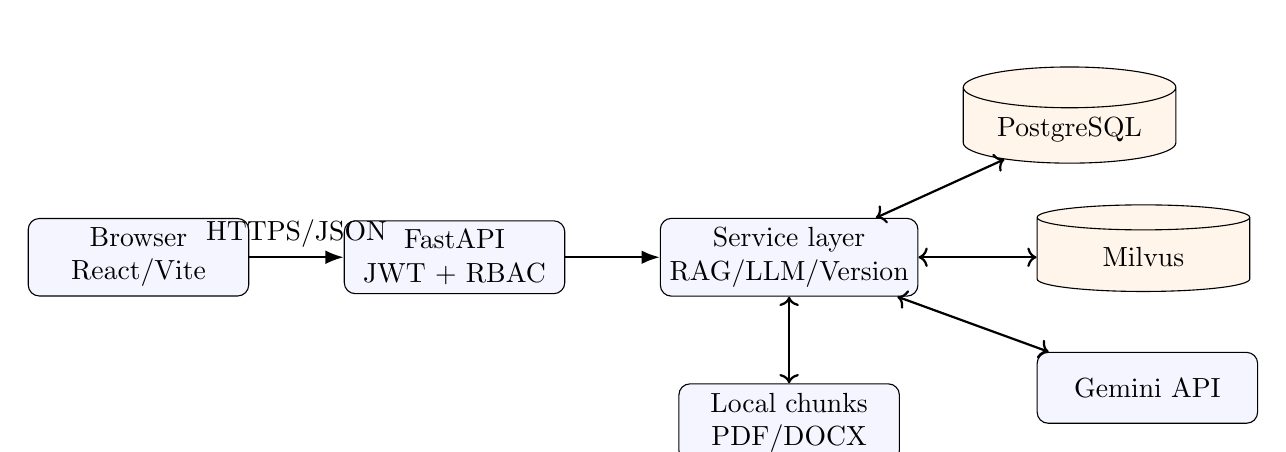
\begin{tikzpicture}[node distance=1.1cm and 1.2cm, box/.style={draw,rounded corners,minimum width=2.8cm,minimum height=0.9cm,align=center,fill=blue!4}, db/.style={cylinder,shape border rotate=90,draw,aspect=0.25,minimum width=2.7cm,minimum height=1.1cm,align=center,fill=orange!8}, arr/.style={-{Latex},thick}]
\node[box] (browser) {Browser\\React/Vite};
\node[box,right=of browser] (api) {FastAPI\\JWT + RBAC};
\node[box,right=of api] (service) {Service layer\\RAG/LLM/Version};
\node[db,above right=0.7cm and 1.5cm of service] (pg) {PostgreSQL};
\node[db,right=1.5cm of service] (milvus) {Milvus};
\node[box,below right=0.7cm and 1.5cm of service] (gemini) {Gemini API};
\node[box,below=1.1cm of service] (files) {Local chunks\\PDF/DOCX};
\draw[arr] (browser)--node[above]{HTTPS/JSON}(api);
\draw[arr] (api)--(service);
\draw[arr,<->] (service)--(pg);
\draw[arr,<->] (service)--(milvus);
\draw[arr,<->] (service)--(gemini);
\draw[arr,<->] (service)--(files);
\end{tikzpicture}}
\caption{Logical architecture of \ProjectName}
\label{fig:architecture}
\end{figure}

\section{Backend Design}
The backend is organized into five main groups. The \code{api} package defines routes and dependencies. The \code{schemas} package defines request and response objects with Pydantic. The \code{crud} package contains database operations. The \code{services} package implements business logic such as LLM orchestration, retrieval, version management, and interview-question generation. The \code{utils} package provides auxiliary functions such as PDF/DOCX export.

This organization keeps endpoint functions concise and avoids mixing HTTP logic with database operations or LLM orchestration. It also allows future developers to replace a component, such as the embedding provider or vector database, without rewriting the entire API layer.

\section{Data Model}
PostgreSQL contains two groups of data. The business group includes \code{users}, \code{roles}, \code{user\_roles}, \code{job\_descriptions}, \code{jd\_versions}, and taxonomy-related tables. The RAG group includes \code{jd\_chunks} and \code{rag\_index\_metadata}. The \code{jd\_chunks} table stores the same \code{chunk\_id} used in Milvus, along with chunk text, heading, hash, path, and token estimate. This allows lexical retrieval and dense retrieval to be merged using a stable key. The manifest records provider, model, dimension, chunker version, and chunk count. Before dense retrieval, the runtime configuration is checked against the manifest to prevent mixing incompatible vector spaces.

\begin{table}[H]
\centering
\caption{Core database tables}
\label{tab:database}
\begin{tabularx}{\textwidth}{p{3.7cm}X}
\toprule
\textbf{Table} & \textbf{Content}\\
\midrule
\code{job\_descriptions} & Current job description, recruitment metadata, provenance, source hash, and version number.\\
\code{jd\_versions} & Markdown snapshots by version, editor, timestamp, and change summary.\\
\code{jd\_chunks} & Chunk text, heading, hash, file path, length, and job-description link.\\
\code{rag\_index\_metadata} & Embedding model, vector dimension, chunker version, document count, and chunk count.\\
\code{users}, \code{roles}, \code{user\_roles} & Account and many-to-many role mapping for RBAC.\\
\code{job\_families}, \code{tags} & Job-family taxonomy and content labels.\\
\bottomrule
\end{tabularx}
\end{table}

\section{Real Job Data Ingestion}
The crawler supports Greenhouse Job Board API, Lever Postings API, and JSON-LD \code{JobPosting}. Each adapter converts source-specific fields into a common structure containing external ID, company, title, description, URL, department, location, employment type, and posting time. The normalized content is stored as Markdown with front matter. SHA-256 hashes are used to detect changes. The ETL process upserts by \code{source\_name} and \code{source\_external\_id}; when the hash does not change, the system updates the observed timestamp instead of creating redundant versions.

The data pipeline follows conservative data-use principles. It collects only public job-posting information through allowed APIs or public pages, uses a clear user agent, respects delay settings, and preserves attribution. It does not access private APIs, bypass CAPTCHA, or collect candidate information. Old synthetic job descriptions are separated from the production-like corpus; the reported experiment uses only 75 real public job descriptions.

\section{RAG Indexing Pipeline}
The chunker prioritizes heading, paragraph, and sentence boundaries. Long blocks are hard-split at word boundaries with overlap. The maximum chunk size is 1,200 characters, and the reported average is 1,007 characters. Embeddings are generated before the index is switched, so quota errors do not leave a partially built index in use. Gemini is called in batches, and the script sleeps between batches according to free-tier limits. After insertion, the Milvus collection is compacted; the PostgreSQL catalog and manifest are updated only after the dense index succeeds.

\begin{figure}[H]
\centering
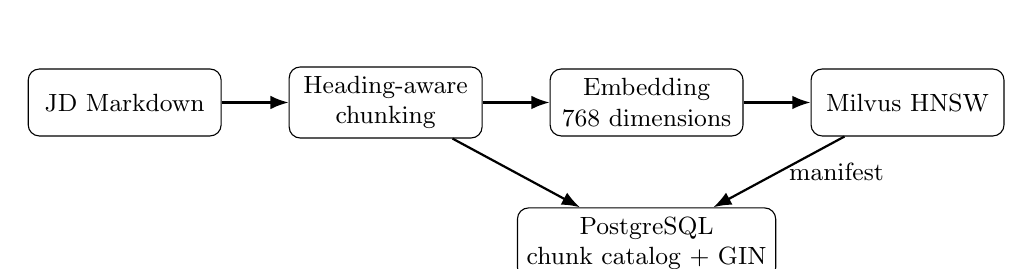
\begin{tikzpicture}[node distance=0.9cm and 0.85cm, every node/.style={font=\small}, box/.style={draw,rounded corners,minimum width=2.45cm,minimum height=0.85cm,align=center}, arr/.style={-{Latex},thick}]
\node[box] (jd) {JD Markdown};
\node[box,right=of jd] (chunk) {Heading-aware\\chunking};
\node[box,right=of chunk] (embed) {Embedding\\768 dimensions};
\node[box,right=of embed] (mv) {Milvus HNSW};
\node[box,below=of embed] (cat) {PostgreSQL\\chunk catalog + GIN};
\draw[arr] (jd)--(chunk);
\draw[arr] (chunk)--(embed);
\draw[arr] (embed)--(mv);
\draw[arr] (chunk)--(cat);
\draw[arr] (mv)--node[right]{manifest}(cat);
\end{tikzpicture}
\caption{RAG indexing pipeline}
\label{fig:index-pipeline}
\end{figure}

\section{Hybrid Retrieval Algorithm}
For each query, the system retrieves up to 40 dense candidates and 40 lexical candidates. Dense search can filter valid job-description IDs by company or department before sending an expression to Milvus. Lexical search assigns high weight to title and uses a GIN index on text content. The two lists are merged with Equation \ref{eq:rrf}. The final selection chooses the candidate with the highest effective score:
\begin{equation}
s'(c)=s_{RRF}(c)-0.08\max_{d\in S}J\big(T(c),T(d)\big),
\label{eq:diversity}
\end{equation}
where $J$ is Jaccard similarity over token sets and $S$ is the set of already selected results. By default, no more than two chunks are selected from the same job description, and only one chunk per job description is used when constructing a generation prompt. If embedding fails in hybrid mode, the endpoint degrades to lexical retrieval instead of failing the whole request.

\begin{figure}[H]
\centering
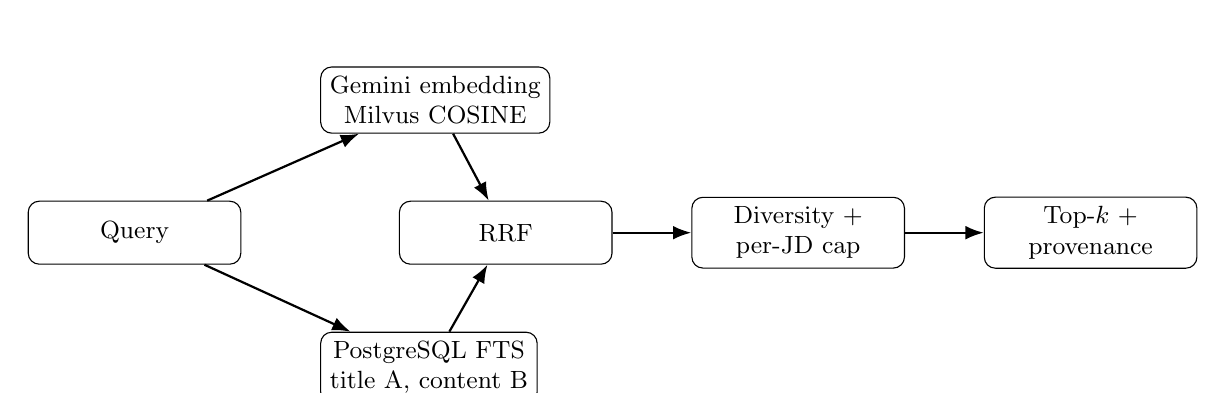
\begin{tikzpicture}[node distance=0.85cm and 1.0cm, every node/.style={font=\small}, box/.style={draw,rounded corners,minimum width=2.7cm,minimum height=0.8cm,align=center}, arr/.style={-{Latex},thick}]
\node[box] (q) {Query};
\node[box,above right=of q] (dense) {Gemini embedding\\Milvus COSINE};
\node[box,below right=of q] (lex) {PostgreSQL FTS\\title A, content B};
\node[box,right=2cm of q] (rrf) {RRF};
\node[box,right=of rrf] (div) {Diversity +\\per-JD cap};
\node[box,right=of div] (out) {Top-$k$ +\\provenance};
\draw[arr] (q)--(dense); \draw[arr] (q)--(lex);
\draw[arr] (dense)--(rrf); \draw[arr] (lex)--(rrf);
\draw[arr] (rrf)--(div); \draw[arr] (div)--(out);
\end{tikzpicture}
\caption{Hybrid retrieval flow}
\label{fig:hybrid}
\end{figure}

\section{LLM Orchestration and Safety}
External job-description content is wrapped in an \code{UNTRUSTED\_SOURCE} block. The prompt instructs the model to extract job-related facts only and to ignore any instruction-like text from the source. The system asks the model to synthesize rather than copy long passages and to keep source URLs visible where appropriate. If the LLM returns a quota or service error, JD generation returns a minimal deterministic template, improvement keeps the original content, and interview-question generation uses an offline fallback with a deterministic seed.

\section{Frontend Design}
The frontend includes Dashboard, Compose, Interview, Retrieve, and Roles pages. The Compose page is the central working area. It contains a metadata form, a Markdown editor, a sanitized preview using DOMPurify, version history, export actions, and an AI Suggestions panel. The Retrieve page allows users to select Hybrid, Dense, or Lexical retrieval and displays score, method, company, title, URL, chunk path, and snippet. The interface supports both English and Vietnamese generation through a language selector.

\section{Deployment Preparation}
The backend is containerized with Docker and can be pushed to AWS Elastic Container Registry. In local development, environment variables are loaded from a \code{.env} file. For cloud deployment, secrets such as database credentials, JWT secret, and Gemini API key should be stored in AWS Systems Manager Parameter Store or AWS Secrets Manager and injected into ECS Task Definitions or EKS Deployments. This avoids hard-coding secrets in source code or container images.

% ============================== CHAPTER 5 ==============================
\chapter{IMPLEMENTATION, TESTING, AND EVALUATION}

\section{Experimental Environment}
The experiments were conducted in a development environment using Python 3.12, Node.js, and Docker Desktop. PostgreSQL 15, Milvus, etcd, and internal object storage components were run with Docker Compose. The backend and frontend were run directly during development to simplify debugging. The embedding model was \code{gemini-embedding-001}, the vector dimension was 768, and the Milvus collection used HNSW with cosine similarity.

\begin{table}[H]
\centering
\caption{Experimental corpus statistics}
\label{tab:corpus}
\begin{tabular}{lr}
\toprule
\textbf{Metric} & \textbf{Value}\\
\midrule
Number of companies & 3\\
Number of public JDs & 75\\
Cloudflare / Datadog / Figma JDs & 25 / 25 / 25\\
Number of chunks & 589\\
Average chunk length & 1,007 characters\\
Maximum chunk length & 1,200 characters\\
Vector dimension & 768\\
\bottomrule
\end{tabular}
\end{table}

\section{Retrieval Evaluation Method}
The \code{evaluate\_rag.py} script selected the first 15 real job descriptions and used each title as a query. The original job description was treated as the relevant document. For a top-$k$ result list, Recall@$k$ measures the percentage of queries for which the relevant document appears in the top-$k$ results. Mean Reciprocal Rank is defined as
\begin{equation}
\operatorname{MRR}=\frac{1}{|Q|}\sum_{q\in Q}\frac{1}{\operatorname{rank}_q}.
\label{eq:mrr}
\end{equation}
The unique JD ratio measures the number of distinct job descriptions divided by the number of returned results. The benchmark was run with at most one chunk per job description in the final top-5 list in order to measure document coverage.

\section{Retrieval Results}
\begin{table}[H]
\centering
\caption{Results on 15 self-retrieval queries, top-$k=5$}
\label{tab:retrieval-result}
\begin{tabular}{lccc}
\toprule
\textbf{Method} & \textbf{Recall@5} & \textbf{MRR} & \textbf{Unique JD ratio}\\
\midrule
Lexical after hyphen normalization & 1.0000 & 1.0000 & 1.0000\\
Dense & 1.0000 & 0.9556 & 1.0000\\
Hybrid RRF & 1.0000 & 0.9556 & 1.0000\\
\bottomrule
\end{tabular}
\end{table}

Before diversity control, the observed top-10 results of several queries contained only 8 or 9 unique job descriptions because one job could occupy multiple positions. After applying the per-JD cap, the top-5 benchmark achieved a unique ratio of 1.0. Lexical retrieval initially missed titles containing hyphens because \code{websearch\_to\_tsquery} interpreted the hyphen as a negation operator. Normalizing separator characters improved lexical Recall@5 and MRR from 0.8 to 1.0. This result shows the value of error analysis beyond simply changing models.

Dense and hybrid retrieval had lower MRR than lexical retrieval on this title-based self-retrieval benchmark because the title is an almost perfect keyword signal. This does not prove that lexical retrieval is better for natural user queries. Dense and hybrid retrieval are expected to be more useful when users describe a role by responsibilities, skills, or business intent rather than by the exact title. An expert-labeled benchmark is needed to verify that expectation.

\section{Software Testing}
\begin{table}[H]
\centering
\caption{Software testing results}
\label{tab:test-result}
\begin{tabularx}{\textwidth}{p{4cm}Xr}
\toprule
\textbf{Group} & \textbf{Content} & \textbf{Result}\\
\midrule
Chunking & Empty input, long block, size limit, and content preservation & Passed\\
Milvus schema & Collection and required fields & Passed\\
Lexical retrieval & Relevance and diversity & Passed\\
Metadata filter & Company-based filtering & Passed\\
Backend E2E & Login, /auth/me, versioning, export, retrieval, and interview fallback & Passed\\
Frontend & Vite production build & Passed\\
Dependency audit & npm audit & 0 vulnerabilities\\
\bottomrule
\end{tabularx}
\end{table}

In the final local measurement, the automated backend tests reported \code{5 passed}. The frontend production build completed successfully, and npm audit reported no known vulnerabilities. PostgreSQL full-text search used a Bitmap Index Scan on the GIN index, and a sample query such as ``sales account executive'' completed in sub-millisecond time in the local environment.

\section{Discussion and Validity Threats}
The corpus has real provenance but remains small and includes only three technology companies. Therefore, the distribution of job titles, languages, and locations is not representative of the entire labor market. The self-retrieval benchmark using titles is biased toward lexical search and does not measure relevance from the perspective of HR experts. High recall also does not directly imply high quality of the generated job descriptions. Furthermore, the LLM is an external service subject to quota limits and temporary service errors. The fallback mechanisms preserve system behavior, but their output quality is lower than full LLM generation.

To reduce these threats, the system records manifest information, timestamps, source URLs, and reproducible benchmark scripts. The reported results should therefore be interpreted as evidence that the prototype is operational and testable, not as a general conclusion about all recruitment domains.

% ============================== CHAPTER 6 ==============================
\chapter{CONCLUSION AND FUTURE WORK}

\section{Conclusion}
This project developed \ProjectName, a RAG-enhanced web system for job-description authoring and interview-question generation. The system supports authentication and RBAC, job-description generation, Markdown editing and preview, version history, PDF/DOCX export, interview-question generation, public job-data ingestion with provenance, vector indexing, and dense/lexical/hybrid retrieval. From a technical perspective, the system connects PostgreSQL and Milvus through stable chunk identifiers, checks embedding compatibility through a manifest, improves retrieval diversity, and applies prompt-safety measures when using external source text.

The experimental corpus contains 75 real public job descriptions and 589 chunks. On a 15-query self-retrieval benchmark, all three retrieval modes achieved Recall@5 of 1.0 after the lexical normalization and diversity improvements. Five automated backend tests passed, and the frontend build completed successfully. The most important result of Project 1 is not only a user interface that calls an LLM, but a traceable and testable data pipeline from source ingestion to retrieval and generation.

\section{Limitations}
The current system still has several limitations. It does not yet include expert-labeled relevance judgments, a rubric-based evaluation of generated job descriptions, a production scheduler for crawlers, fully incremental vector updates, automatic detection of closed job postings, multi-tenant data isolation, cloud secret management, HTTPS termination, distributed tracing, or large-scale load testing. The local lexical fallback is based on hashing and should not be considered equivalent to semantic embeddings.

\section{Future Work}
Future development can proceed in four directions. First, the project should build an expert-labeled evaluation set with natural-language HR queries, relevance judgments, and a generation-quality rubric. Second, the retrieval pipeline can be improved with a cross-encoder reranker, query expansion, and learning-to-rank, followed by A/B testing of RRF weights. Third, the data pipeline should support scheduled crawling, hash-based incremental indexing, closed-posting detection, and retention policies. Fourth, production readiness should be improved with HTTPS, secret management, OpenTelemetry, Redis caching, worker queues, PostgreSQL backup, and load testing. In the recruitment domain, future versions should also include bias checking, inclusive-language review, and human-in-the-loop approval before generated content is published.

% ============================== REFERENCES ==============================
\begin{thebibliography}{99}
\addcontentsline{toc}{chapter}{References}

\bibitem{lewis2020rag}
P. Lewis et al., ``Retrieval-Augmented Generation for Knowledge-Intensive NLP Tasks,'' \textit{Advances in Neural Information Processing Systems}, vol. 33, 2020.

\bibitem{cormack2009rrf}
G. V. Cormack, C. L. A. Clarke, and S. Buettcher, ``Reciprocal Rank Fusion Outperforms Condorcet and Individual Rank Learning Methods,'' \textit{Proceedings of SIGIR}, 2009.

\bibitem{carbonell1998mmr}
J. Carbonell and J. Goldstein, ``The Use of MMR, Diversity-Based Reranking for Reordering Documents and Producing Summaries,'' \textit{Proceedings of SIGIR}, 1998.

\bibitem{malkov2018hnsw}
Y. A. Malkov and D. A. Yashunin, ``Efficient and Robust Approximate Nearest Neighbor Search Using Hierarchical Navigable Small World Graphs,'' \textit{IEEE Transactions on Pattern Analysis and Machine Intelligence}, vol. 42, no. 4, 2020.

\bibitem{rfc7519}
M. Jones, J. Bradley, and N. Sakimura, ``JSON Web Token (JWT),'' RFC 7519, IETF, 2015. \url{https://www.rfc-editor.org/rfc/rfc7519}

\bibitem{geminiembed}
Google, ``Gemini Embeddings,'' Google AI for Developers. \url{https://ai.google.dev/gemini-api/docs/embeddings}, accessed June 2026.

\bibitem{milvusdocs}
Milvus, ``Milvus Documentation: Vector Search and HNSW Index.'' \url{https://milvus.io/docs}, accessed June 2026.

\bibitem{pgfts}
PostgreSQL Global Development Group, ``PostgreSQL Full Text Search.'' \url{https://www.postgresql.org/docs/15/textsearch.html}, accessed June 2026.

\bibitem{fastapi}
FastAPI, ``FastAPI Documentation.'' \url{https://fastapi.tiangolo.com/}, accessed June 2026.

\bibitem{greenhouse}
Greenhouse Software, ``Job Board API.'' \url{https://developers.greenhouse.io/job-board.html}, accessed June 2026.

\bibitem{lever}
Lever, ``Lever Postings API.'' \url{https://github.com/lever/postings-api}, accessed June 2026.

\bibitem{schemajob}
Schema.org, ``JobPosting.'' \url{https://schema.org/JobPosting}, accessed June 2026.
\end{thebibliography}

% ============================== APPENDICES ==============================
\appendix
\chapter{INSTALLATION AND OPERATION GUIDE}
\label{app:install}

\section{Environment Setup}
\begin{lstlisting}[language=bash,caption={Environment setup commands on Windows PowerShell}]
py -3.12 -m venv .venv
.\.venv\Scripts\python.exe -m pip install -r requirements.txt
cd frontend
npm ci
cd ..
.\scripts\bootstrap.ps1
\end{lstlisting}

\section{Running the Application}
\begin{lstlisting}[language=bash,caption={Running backend and frontend}]
# Backend
$env:PYTHONUTF8="1"
.\.venv\Scripts\python.exe -m uvicorn src.main:app --host 0.0.0.0 --port 8000

# Frontend
cd frontend
npm run dev -- --host 0.0.0.0
\end{lstlisting}

\section{Crawling, ETL, and Indexing}
\begin{lstlisting}[language=bash,caption={Data ingestion and indexing commands}]
.\.venv\Scripts\python.exe scripts\crawl_jobs.py ^
  --source greenhouse --site cloudflare ^
  --company Cloudflare --limit 25

.\.venv\Scripts\python.exe etl\jd_etl.py ^
  --dir data\real_jd --author public-api-ingestion

.\.venv\Scripts\python.exe embeddings\jd_chunk_embed.py
\end{lstlisting}

\chapter{MAIN API LIST}
\label{app:api}
\begin{longtable}{p{2cm}p{5.4cm}p{7cm}}
\toprule
\textbf{Method} & \textbf{Endpoint} & \textbf{Purpose}\\
\midrule
POST & \code{/auth/token} & Log in and receive a JWT.\\
GET & \code{/auth/me} & Retrieve the current user profile.\\
POST & \code{/v1/jd/generate} & Generate a job description, optionally with RAG context.\\
PUT & \code{/v1/jd/update} & Save a new version of a job description.\\
GET & \code{/v1/jd/version-history/\{id\}} & List versions of a job description.\\
POST & \code{/v1/jd/improve} & Improve an existing job description.\\
POST & \code{/v1/jd/suggest} & Suggest content for a selected JD section.\\
GET & \code{/v1/jd/export/\{id\}} & Export a JD to PDF or DOCX.\\
POST & \code{/v1/interview/generate} & Generate interview questions.\\
POST & \code{/v1/retrieve} & Hybrid, dense, or lexical retrieval.\\
POST & \code{/v1/retrieve/similar} & Dense retrieval compatible with the older API.\\
GET & \code{/health/live} & Liveness check.\\
GET & \code{/health/ready} & Readiness check for storage and index.\\
\bottomrule
\end{longtable}

\chapter{SOURCE CODE STRUCTURE}
\begin{lstlisting}[caption={Main source-code structure}]
Project1/
|-- src/                 # FastAPI, services, ORM, schemas
|-- frontend/            # React/Vite frontend
|-- embeddings/          # chunking, embedding, indexing
|-- etl/                 # Markdown -> PostgreSQL ETL
|-- scripts/             # crawler, benchmark, bootstrap
|-- infra/migrations/    # PostgreSQL migrations
|-- data/real_jd/        # public JDs with provenance
|-- data/chunks/         # local chunk Markdown files
|-- tests/, test/        # automated tests
`-- report/              # LaTeX report
\end{lstlisting}

\chapter{REPRESENTATIVE TEST CASES}
\begin{longtable}{p{1.3cm}p{4.8cm}p{5.2cm}p{3.3cm}}
\toprule
\textbf{ID} & \textbf{Precondition / Data} & \textbf{Action} & \textbf{Expected Result}\\
\midrule
T01 & User \code{hr\_admin} is seeded & POST \code{/auth/token} & A valid Bearer JWT is returned.\\
T02 & Recruiter JWT exists & Create a new JD & JD and version 1 are saved.\\
T03 & A JD exists & Update twice & Version numbers increase sequentially, history is ordered from newest to oldest.\\
T04 & Milvus and catalog are synchronized & Query ``sales account executive'' & Top-5 results are relevant and do not repeat the same JD.\\
T05 & Gemini embedding fails temporarily & Hybrid retrieval & The system falls back to lexical retrieval without breaking the API.\\
T06 & Company filter = Figma & Retrieve with filter & All returned results belong to Figma.\\
T07 & Content contains special characters & Export PDF/DOCX & HTTP 200 is returned and the file can be opened.\\
T08 & Milvus collection is missing & GET readiness & HTTP 503 is returned with index check = false.\\
\bottomrule
\end{longtable}

\end{document}
